%!TEX output_directory = .cache

\documentclass[12pt]{letter}
\usepackage[utf8]{inputenc}
\usepackage{graphicx}
\usepackage{eurosym}
\usepackage{charter}
\usepackage{hyperref}  
\usepackage{xcolor}  

\hypersetup{
    colorlinks,
    linkcolor=[HTML]{404040},
    urlcolor={red!50!black}
}

\signature{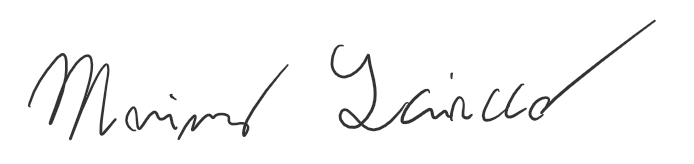
\includegraphics[scale=0.6]{images/mariano} 
			Mariano Sciacco  \\ 
			\textit{Responsabile di progetto}
			\href{mailto:redroundrobin.site@gmail.com}{redroundrobin.site@gmail.com}}
\address{ Via Trieste 63 \\ Padova \\ PD 35121, Italia}

\date{14 gennaio 2020}

\begin{document}

\begin{letter}{ }


\includegraphics[scale=0.17]{images/logo.png}

\opening{Gentile prof. Vardanega,\\ Gentile prof. Cardin, }

con la presente il gruppo 6, \textit{Red Round Robin}, vuole confermare la volontà di realizzazione del prodotto da Voi commissionato dal titolo 
\textbf{ThiReMa Project (Capitolato 6)}, proposto dall'azienda \textit{San Marco Informatica}. Inoltre, comunichiamo che i costi preventivati per lo sviluppo del prodotto sono pari a \EUR{}13.806,00.

Le forniamo il link di una repository pubblica da cui è possibile scaricare e visualizzare online i documenti richiesti dal progetto.
In particolare:

\begin{itemize}
	\item \textit{Analisi dei Requisiti v1.0.0+b0.4};
	\item \textit{Piano di Qualifica v1.0.0+b0.4};
	\item \textit{Piano di Progetto v1.0.0+b0.4};
	\item \textit{Norme di Progetto v1.0.0+b0.4};
	\item \textit{Studio di Fattibilità v1.0.0+b0.4};
	\item \textit{Glossario v1.0.0+b0.4};
	\item \textit{verbali interni};
	\item \textit{verbali esterni}.
\end{itemize}

Il link per scaricare e visualizzare i documenti è il seguente:

\begin{center}
\href{https://drive.google.com/open?id=17qt131a_wV08n1jLR0fiSS8FoROeKiSY}{http://rr.redroundrobin.site}
\end{center}

\newpage

Per qualunque altro chiarimento o problema, rimaniamo a completa disposizione.

\closing{Cordiali saluti,}


\vspace{3em}
\ps 

\textbf{P.S.} Se il link fornito non dovesse funzionare, potete fare riferimento al seguente link: 
\href{https://www.redroundrobin.site}{www.redroundrobin.site}

\end{letter}

\end{document}